Fig.~\ref{fig:prefetcher_speedup} shows our prefetcher's speedup compared to
running the test without a prefetcher. As you can see from the chart there is
an all-round good speedup, in addition to certain test which have higher
speedup.

As you can see from Fig.~\ref{fig:table_size_chart}, the performance stopped
increasing after a table size of 256. This we believe is caused by instruction
conflicts in the table. When the table reaches a certain size, most
instructions get their own place in the table, and avoid being evicted by
conflicting instructions.

The final solution was selected after thorough testing and tweaking of the
prefetcher. The different results form the tests can be seen in
Fig.~\ref{fig:prefetcher_tweaks}. Each line represents different values for the
threshold, and the x-axis shows the values for the count variable.

\begin{figure}
	\centering 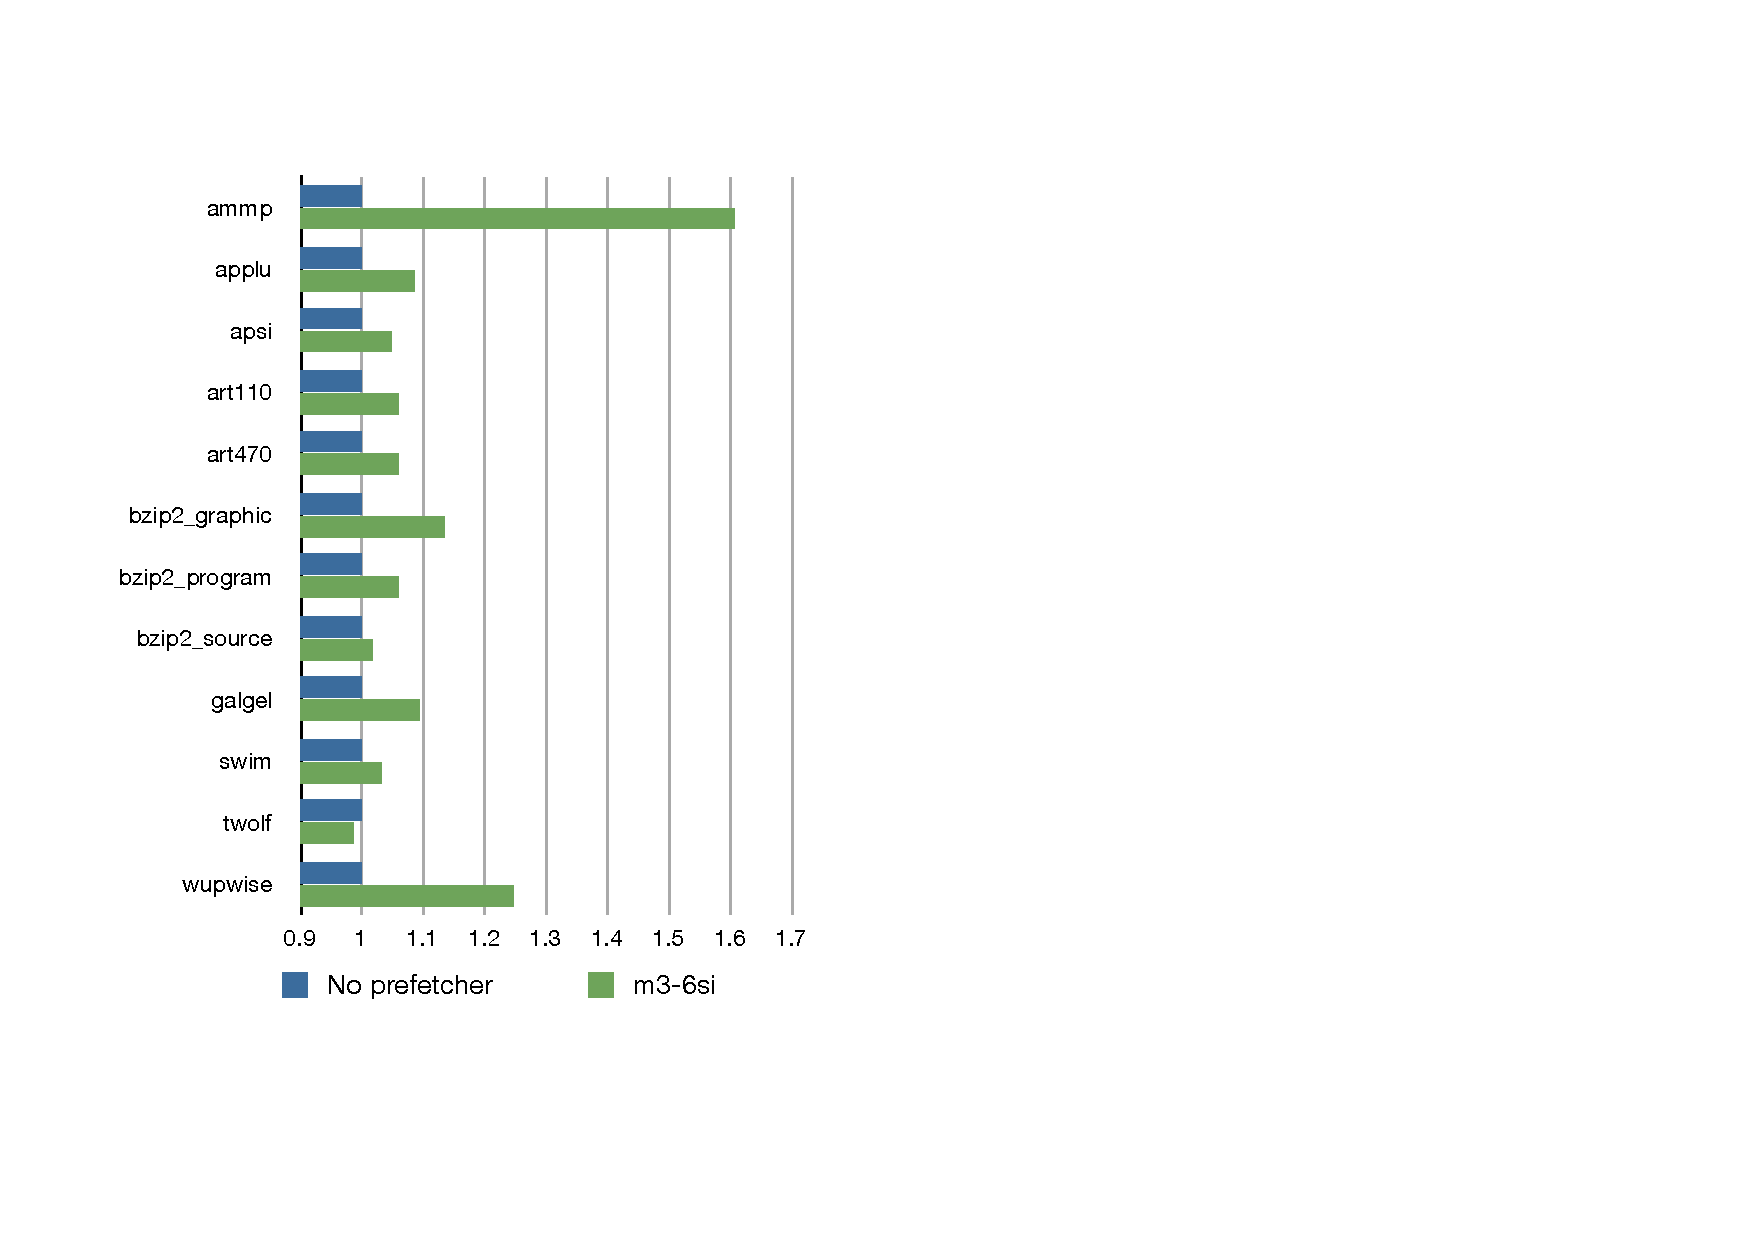
\includegraphics[scale=0.7]{img/prefetcher_chart.pdf}
	\caption{Prefetcher speedup chart}
	\label{fig:prefetcher_speedup}
\end{figure}

\begin{figure}
	\centering 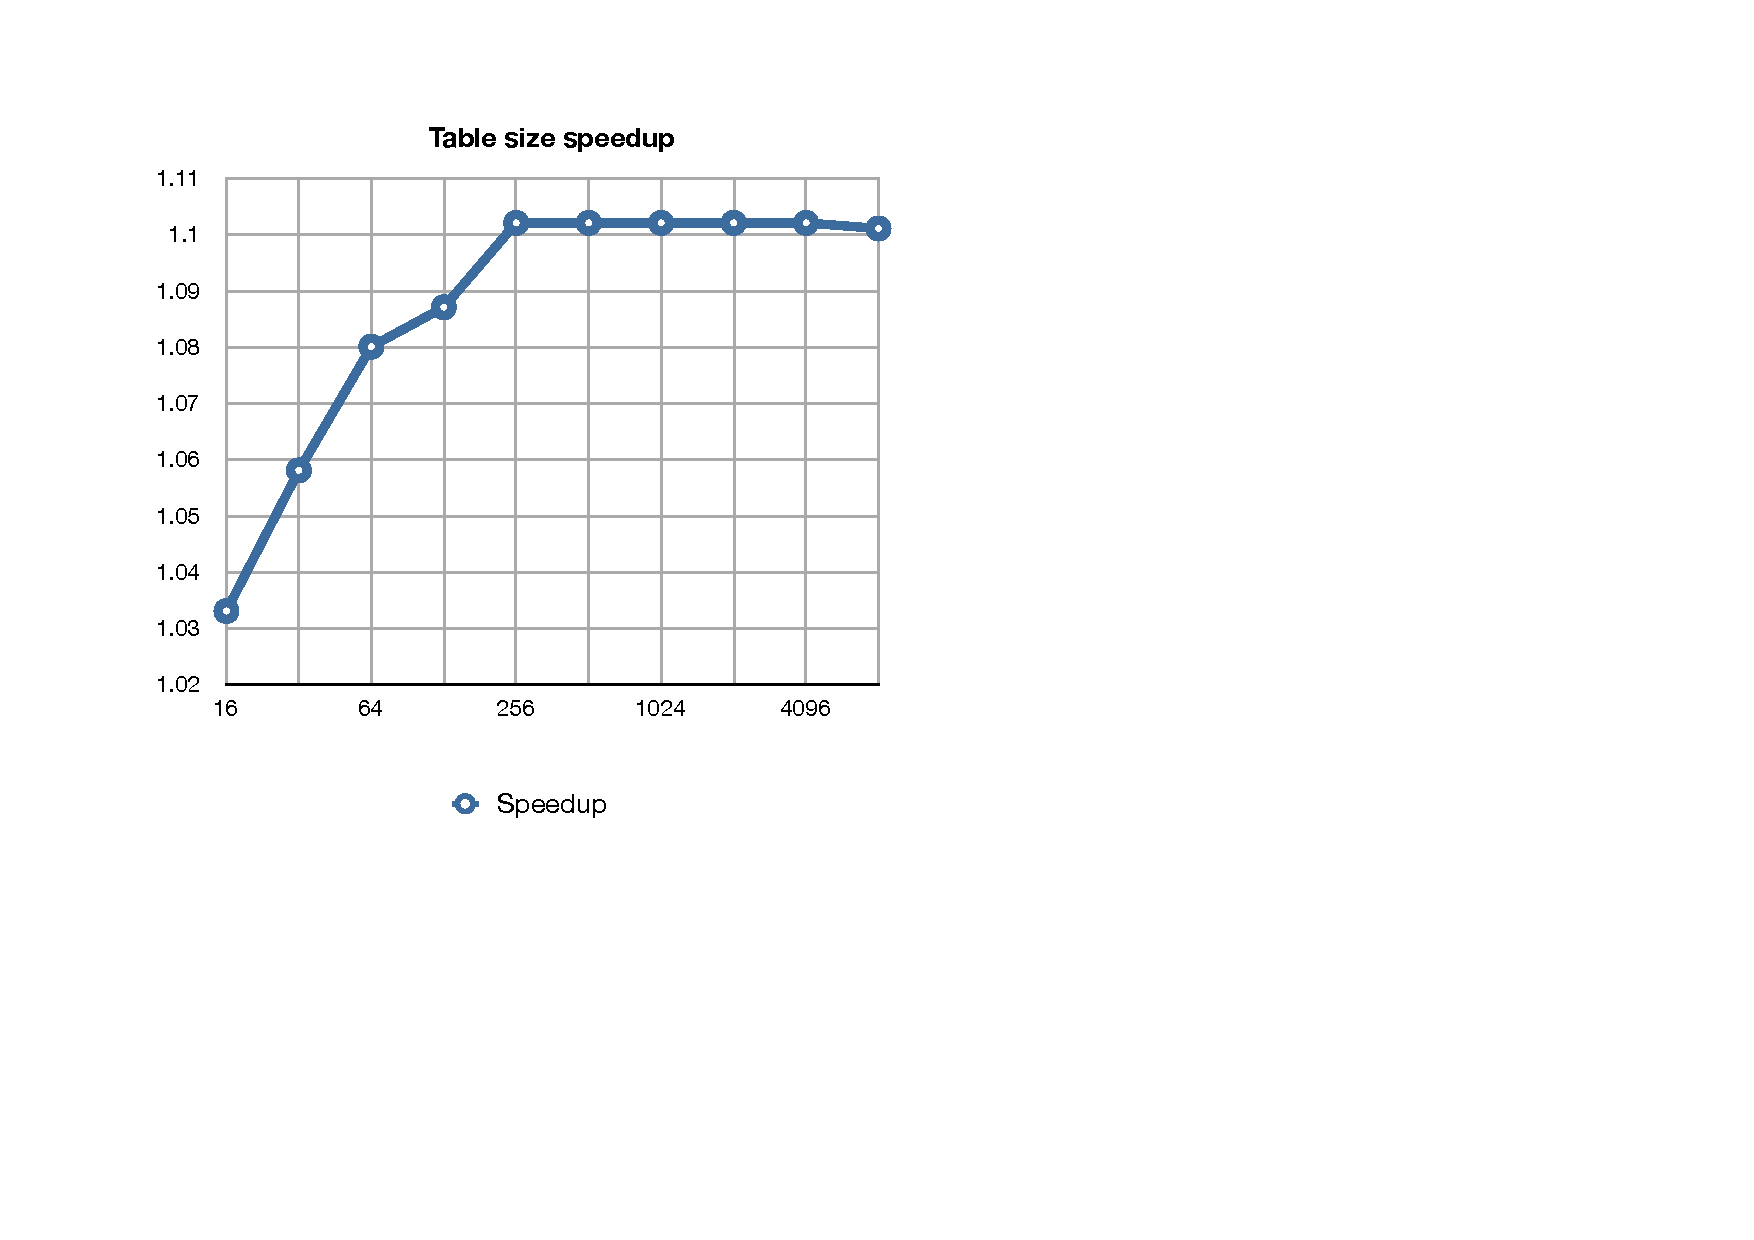
\includegraphics[scale=0.7]{img/table_size_chart.pdf}
	\caption{Table size speedup chart}
	\label{fig:table_size_chart}
\end{figure}

\begin{figure}
	\centering 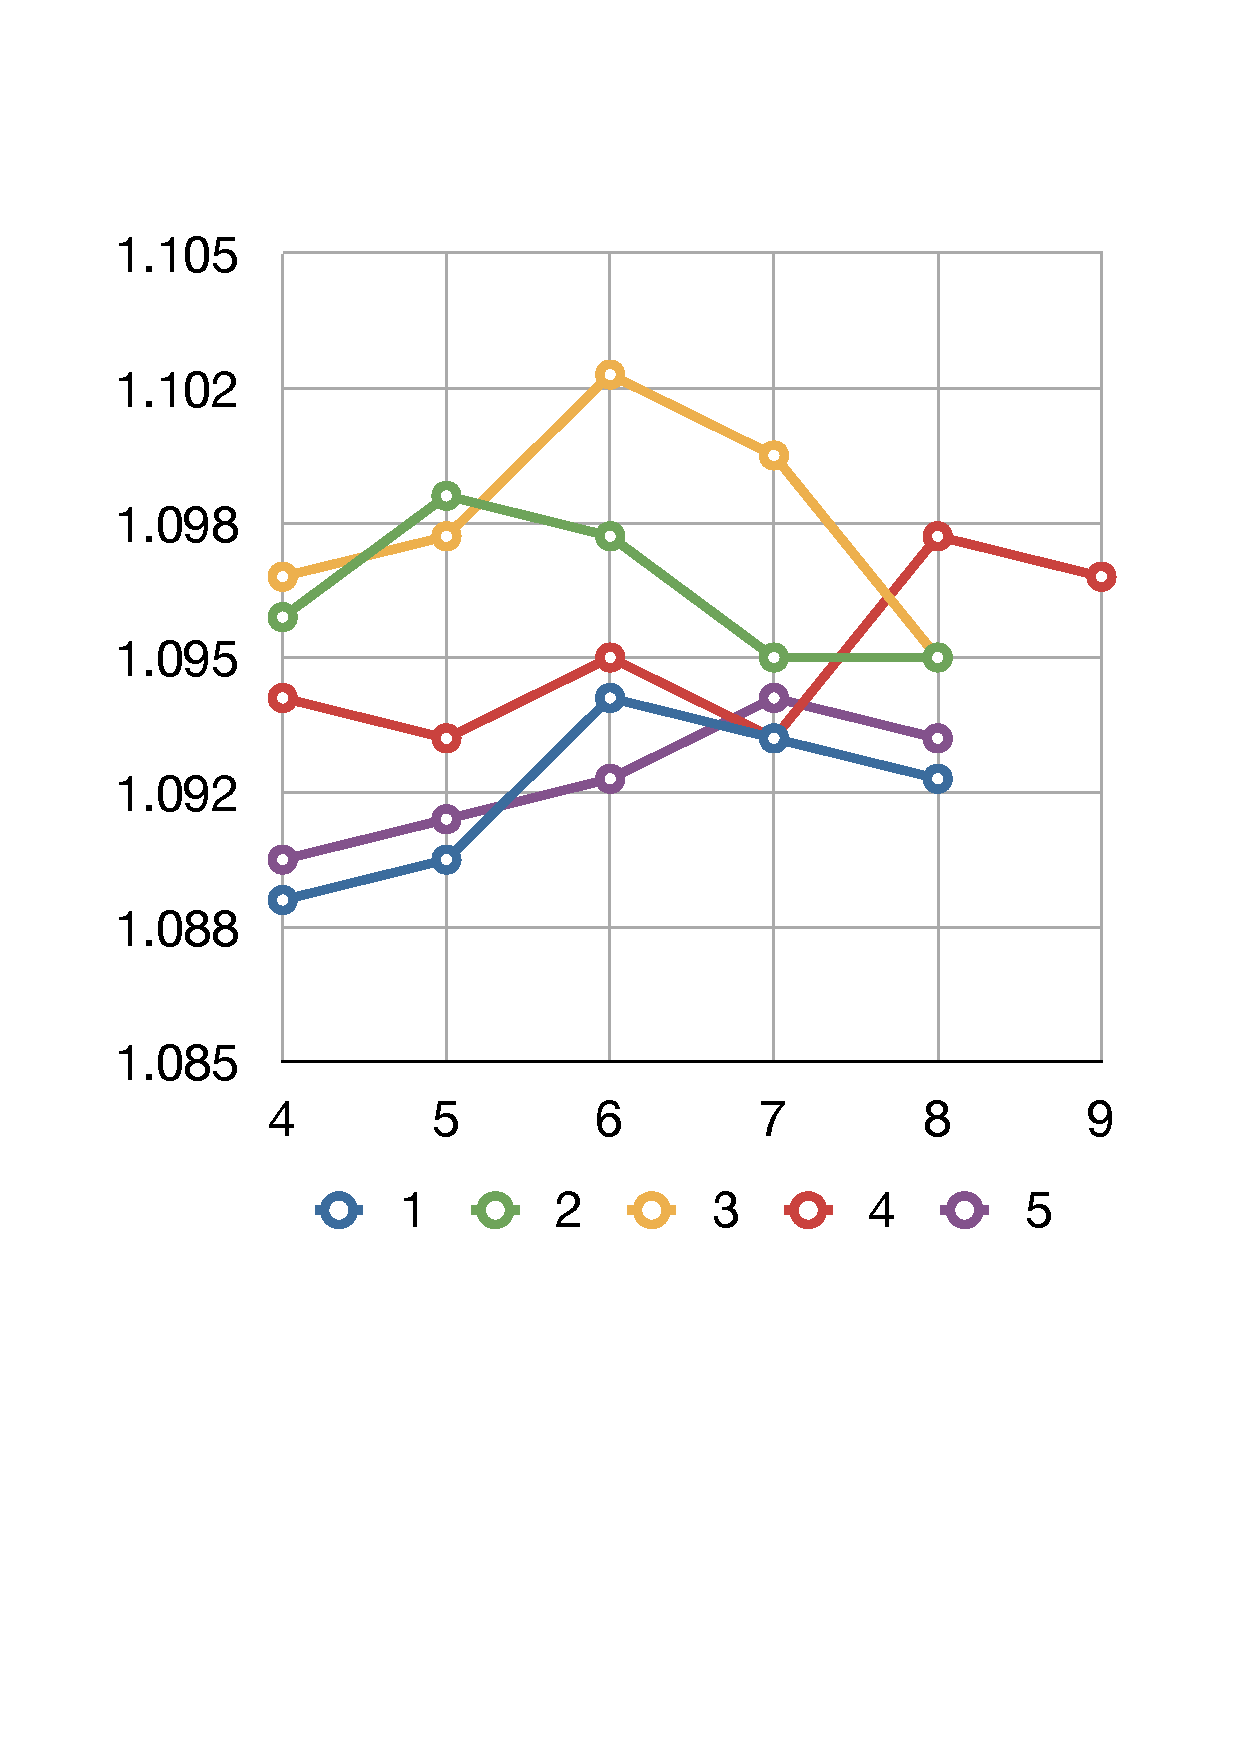
\includegraphics[scale=0.5]{img/prefetcher_tweaks.pdf}
	\caption{Prefetcher tweaks}
	\label{fig:prefetcher_tweaks}
\end{figure}
